\documentclass[11pt,oneside,letterpaper]{article}

% graphicx package, useful for including eps and pdf graphics
\usepackage{graphicx}
\usepackage{grffile}
\usepackage{subfig}
%\DeclareGraphicsExtensions{.pdf,.png,.jpg}

% basic packages
\usepackage{color}
\usepackage{parskip}
\usepackage{float}
\usepackage{microtype}
\usepackage{url}
\urlstyle{same}

\usepackage[hidelinks]{hyperref}
\hypersetup{colorlinks=true,linkcolor=black,citecolor=black,urlcolor=black}

\usepackage{longtable}
\usepackage[]{algorithm2e}

% reference figures across documents
% \usepackage{xr}
% \externaldocument{mers-structure_supp}

% text layout
\usepackage{geometry}
\geometry{textwidth=15cm} % 15.25cm for single-space, 16.25cm for double-space
\geometry{textheight=22cm} % 22cm for single-space, 22.5cm for double-space

% helps to keep figures from being orphaned on a page by themselves
\renewcommand{\topfraction}{0.85}
\renewcommand{\textfraction}{0.1}

% bold the 'Figure #' in the caption and separate it with a period
% Captions will be left justified
\usepackage[labelfont=bf,labelsep=period,font=small]{caption}
% \RequirePackage{subfigure}

% review layout with double-spacing
%\usepackage{setspace}
%\doublespacing
%\captionsetup{labelfont=bf,labelsep=period,font=doublespacing}

% cite package, to clean up citations in the main text. Do not remove.
%\usepackage{cite}
\usepackage{natbib}
%\renewcommand\citepleft{(}
%\renewcommand\citepright{)}
%\renewcommand\citepform[1]{\textsl{#1}}

\usepackage{amsmath}

%\usepackage{lineno}
%\linenumbers

% Remove brackets from numbering in list of References
%\renewcommand\refname{\large References}
%\makeatletter
%\renewcommand{\@biblabel}[1]{\quad#1.}
%\makeatother

\usepackage{authblk}
\renewcommand\Authands{ \& }
\renewcommand\Authfont{\normalsize \bf}
\renewcommand\Affilfont{\small \normalfont}
\makeatletter
\renewcommand\AB@affilsepx{, \protect\Affilfont}
\makeatother

% comments
%\usepackage{ulem}
\definecolor{purple}{rgb}{0.459,0.109,0.538}
\def\tb#1#2{\sout{#1} \textcolor{purple}{#2}}
\def\tbc#1{\textcolor{purple}{[#1]}}
\def\gdc#1{\textcolor{blue}{[#1]}}
\def\lmc#1{\textcolor{green}{[#1]}}

% symbols
% \newcommand{\chiSq}{\chi^{2}_{df}} %LM: ancient DNA? =P %GD: quite :)
% \newcommand{\dtmrca}{\Delta_\mathrm{TMRCA}}
% \newcommand{\undtmrca}{\delta_\mathrm{TMRCA}}
% \newcommand{\dspr}{d_\mathrm{SPR}}

%%% TITLE %%%
\title{\vspace{1.0cm} \LARGE \bf TITLE HERE}

\author[1,2]{Sidney Bell}
\author[3]{Leah Katzelnick}
\author[1]{Trevor Bedford}

\affil[1]{Vaccine and Infectious Disease Division, Fred Hutchinson Cancer Research Center, Seattle, WA, USA}
\affil[2]{Molecular and Cell Biology Graduate Program, University of Washington, Seattle, WA, USA}
\affil[3]{Some Department, University of California, Berkeley, CA, USA}

% \date{\today}

\begin{document}
\maketitle

\begin{abstract}
  % SB: Placeholder copied over from epidemics abstract

  Lorem ipsum dolor sit amet, consectetur adipisicing elit, sed do eiusmod tempor incididunt ut labore et dolore magna aliqua. Ut enim ad minim veniam, quis nostrud exercitation ullamco laboris nisi ut aliquip ex ea commodo consequat. Duis aute irure dolor in reprehenderit in voluptate velit esse cillum dolore eu fugiat nulla pariatur. Excepteur sint occaecat cupidatat non proident, sunt in culpa qui officia deserunt mollit anim id est laborum.

\end{abstract}

\pagebreak

\section*{Introduction}

Lorem ipsum dolor sit amet, consectetur adipisicing elit, sed do eiusmod tempor incididunt ut labore et dolore magna aliqua. Ut enim ad minim veniam, quis nostrud exercitation ullamco laboris nisi ut aliquip ex ea commodo consequat. Duis aute irure dolor in reprehenderit in voluptate velit esse cillum dolore eu fugiat nulla pariatur. Excepteur sint occaecat cupidatat non proident, sunt in culpa qui officia deserunt mollit anim id est laborum.


\section*{Results}

\subsection{Dengue neutralization titer data}
% Figure 1A: titer heat map

\begin{figure}[h]
 \centering
    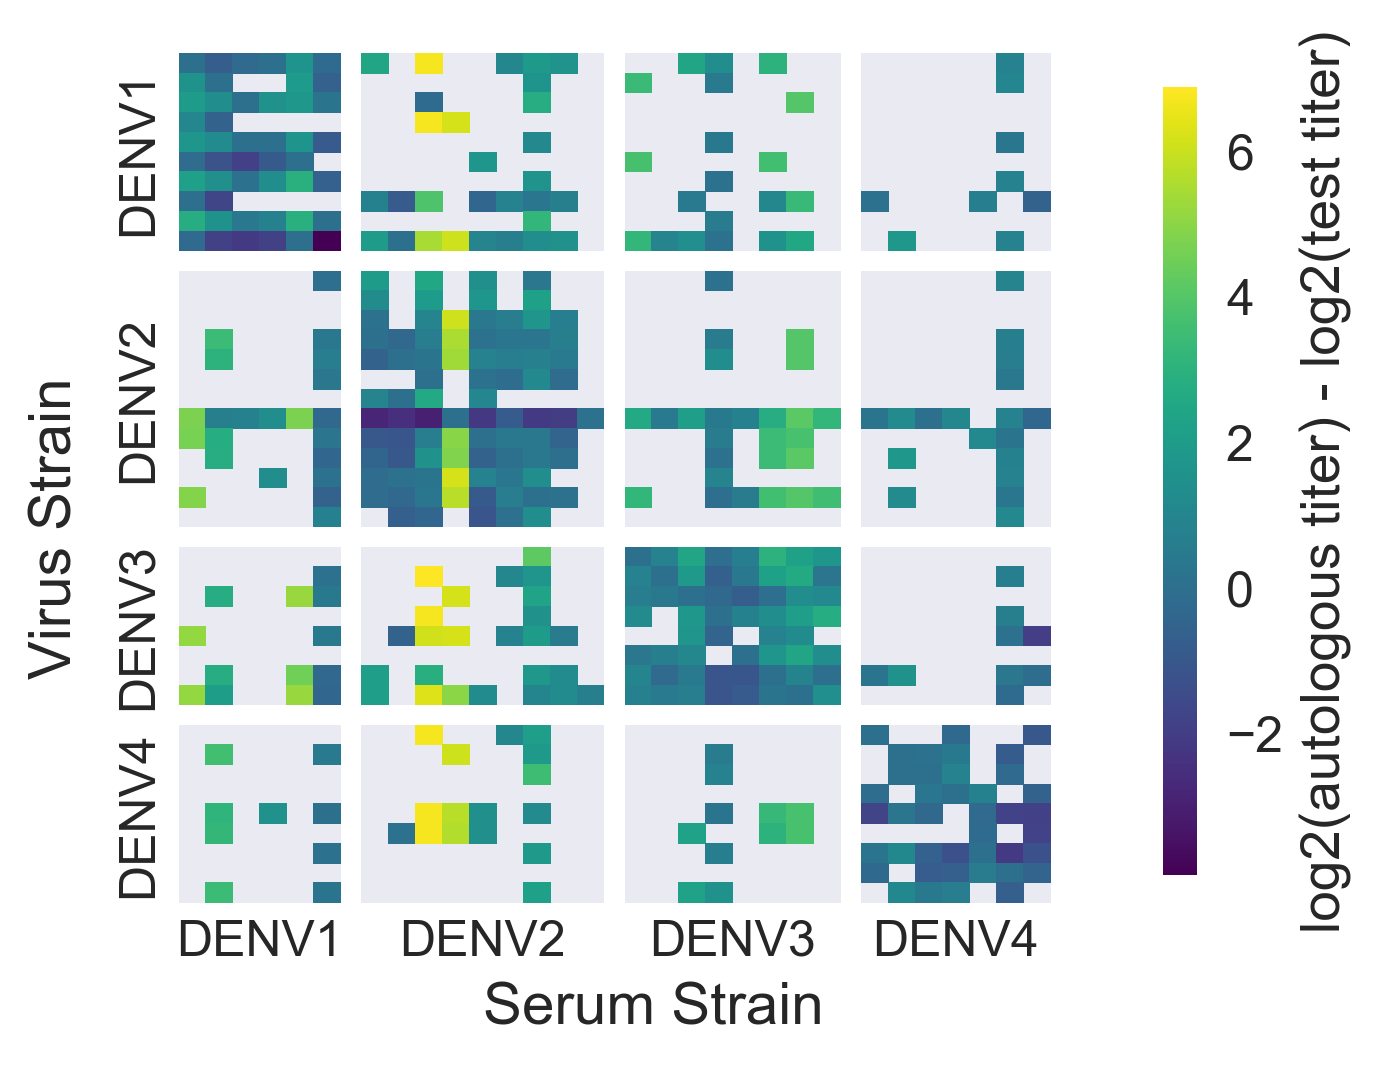
\includegraphics[width=\linewidth]{../figures/png/titer_heatmap.png}
    \caption{\textbf{Normalized antigenic distance between pairs of dengue virus strains and sera.}}
     \label{titer_heatmap}
\end{figure}
\begin{figure}[h]
  \centering 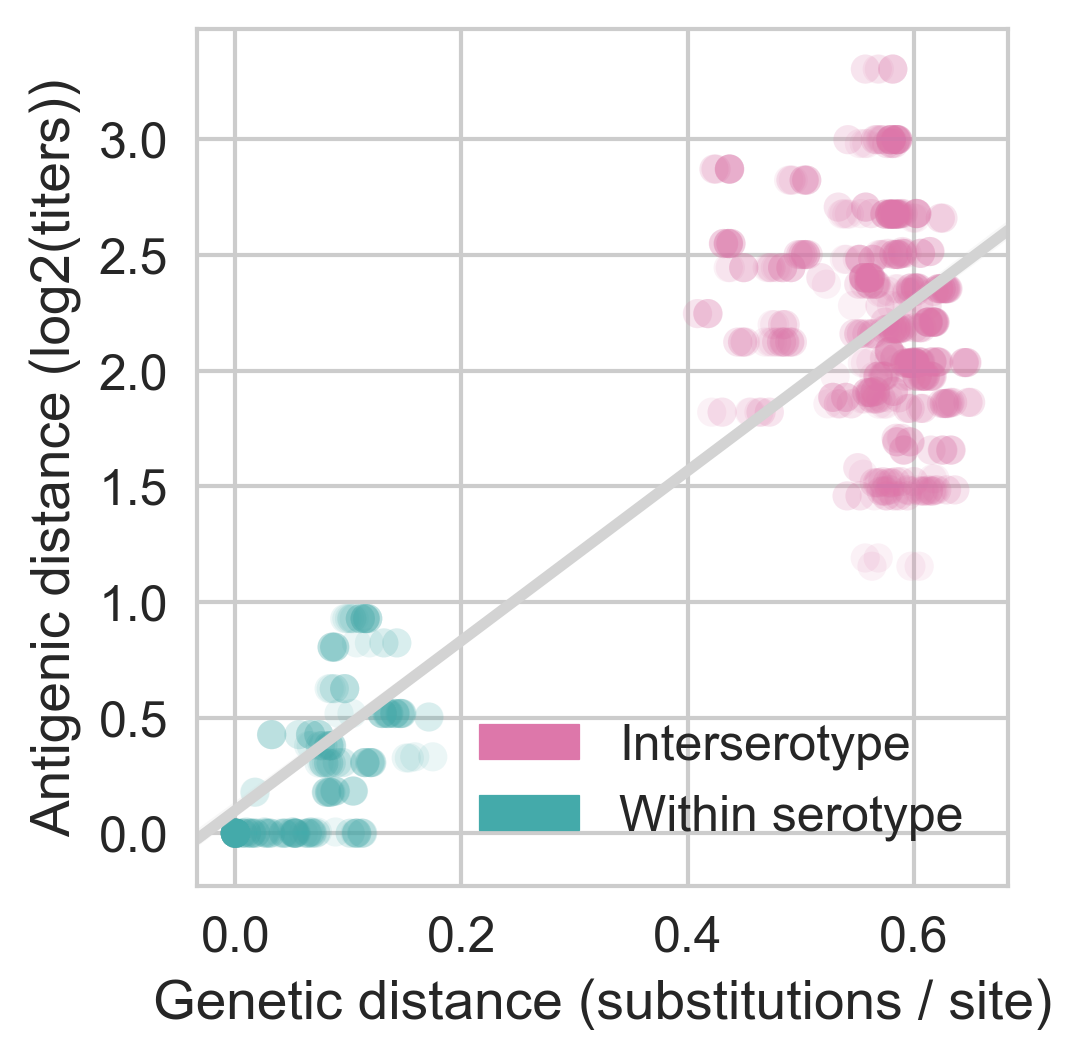
\includegraphics[width=\linewidth]{../figures/png/genetic_antigenic_distance.png}
  	\caption{\textbf{Normalized antigenic distance vs. genetic distance between pairs of dengue strains.}}
  	\label{genetic_antigenic_distance}
\end{figure}

Antigenic distance between pairs of viruses $i$ and $j$ is experimentally measured using a neutralization titer, which measures how well serum drawn after infection with virus $i$ is able to neutralize virus $j$ in vitro.

Briefly, serum $i$ is serially diluted and incubated with a fixed concentration of virus $j$.
Titers represent the lowest serum concentration able to neutralize $50\%$ of virus, and are reported as the inverse dilution.
Thus, a higher titer value indicates that less of serum $i$ is required to neutralize virus $j$, implying stronger cross-neutralization and smaller antigenic distance between viruses $i$ and $j$.
To measure the pairwise antigenic distances for a panel of X strains of DENV, Katzelnick et al. infected naive non-human primates (NHP) with each virus, drew sera at 3 months post-infection, and then titered this sera against each virus in the panel.
To compare patterns of cross-protection in NHP and humans, they also drew sera from X study participants 6 weeks after infection with a monovalent component of the NIH dengue vaccine candidate.
This sera was also titered against the same panel of X DENV strains.
Together, these X measurements make up our dataset.

To normalize these measurements, we first take the $log_2$ of each value, such that one titer unit corresponds to one 2-fold dilution of sera.
We then define antigenic distance between autologous virus-sera pairs (i.e., virus $i$ and serum $i$) as 0.
Normalized titers between $i$ and $j$ are thus calculated as $T_{ij} = log_2(T_{ij}) - log_2(T_{ii})$.

The full dataset of normalized titer values is shown in Figure ~\ref{titer_heatmap}.
Here, we see that homotypic virus-serum pairs are more closely related antigenically than heterotypic pairs.
However, we also observe large variance around this trend, both within and between serotypes.
This suggests that treating each serotype as antigenically uniform overlooks potentially important antigenic heterogeneity across strains within each serotype.

\subsection{Dengue antigenic evolution corresponds to phylogenetic divergence}
%Figure 1B: genetic vs. antigenic divergence

Titer measurements are prone to noise, and there is a limited amount of available data.
If the antigenic heterogeneity observed in the raw data is truly the result of an underlying evolutionary process, we expect changes in antigenic phenotype to be driven by underlying changes in viral genotype.
Figure ~\ref{genetic_antigenic_distance} shows the relationship between genetic (patristic) and antigenic distance between each pair of viruses in our dataset.
Notably, increasing genetic divergence generally corresponds to increased antigenic distance, both within and between serotypes.

\subsection{Within-serotype antigenic evolution better explains observed antigenic relationships}
%Figure 2: titer model formulations + performance
We then sought to fully map the relationship between DENV genetic and antigenic evolution.
To do so, we adapted a phylogenetics-based model originally developed for influenza. %neher et al reference
Conceptually, this model predicts titer values through three steps (see Methods for detailed formulas).
First, we build a phylogeny of dengue virus sequences to establish the genetic relationships between viruses.
Next, we infer how much antigenic change has occurred along each branch of the phylogeny (denoted $d_b$).
Finally, once each branch has been assigned a $d_b$ value, we can estimate the titer distance between any pair of viruses by tracing the path between them in the phylogeny, summing values of $d_b$ as we go.

To learn these values of $d_b$, we first split our dataset into training (random 90\% of measurements) and test data (the remaining 10\% of values).
The model then tries to infer one value of $d_b$ for each branch in the tree, subject to a few constraints.
Parsimoniously, we expect that antigenic change is more likely to occur through fewer, larger changes than through many small changes; correspondingly, values of $d_b$ are exponentially distributed such that most values of $d_b = 0$.
Additionally, some viruses have greater binding avidity, and some sera are more potent than others; these row and column effects, respectively, are normally distributed and are taken into account when estimating titers.
The model uses convex optimization to learn the values of $d_b$ that minimize the sum of squared error (SSE) between observed and predicted titers in the training data.

This model is a powerful tool for estimating antigenic relationships between viruses based on their relative positions in the phylogeny.
We can also use variations of this model to explicitly test whether the observed antigenic phenotypes are better explained by the hypothesis that dengue serotypes are antigenically uniform ("interserotype model"), or by the hypothesis that serotypes are antigenically diverse ("full tree model").

We find that serotype-level characterization is insufficient to explain observed antigenic phenotypes.
In the interserotype model, we set $d_b = 0$ for all branches in the tree that do not lie between serotypes.
On average, this interserotype model predicts titers within a $2.4$-fold dilution of the true value, and explains $22\%$ of the observed variation in neutralization titers overall.

We find that accounting for within-serotype antigenic evolution substantially improves our ability to explain dengue antigenic phenotypes.
When we allow any branch in the phylogeny to contribte to antigenic evolution, this full tree model is able to predict test titers within a $1.9$-fold dilution of the true value (approaching the level of error intrinsic to the assay), and explains $66\%$ of the observed variation in neutralization titers overall.
Importantly, all reported error metrics refer to performance on test data, so this difference in model performance is not due to the number of free parameters.
The full tree model performance is comparable to the model error from a cartography-based characterization of the same dataset, and to the error observed when this model was used to characterize an influenza dataset.
From this, we conclude that there is significant antigenic evolution within each serotype of DENV, and that this is driven by underlying genetic divergence.

\begin{figure}[h]
\centering
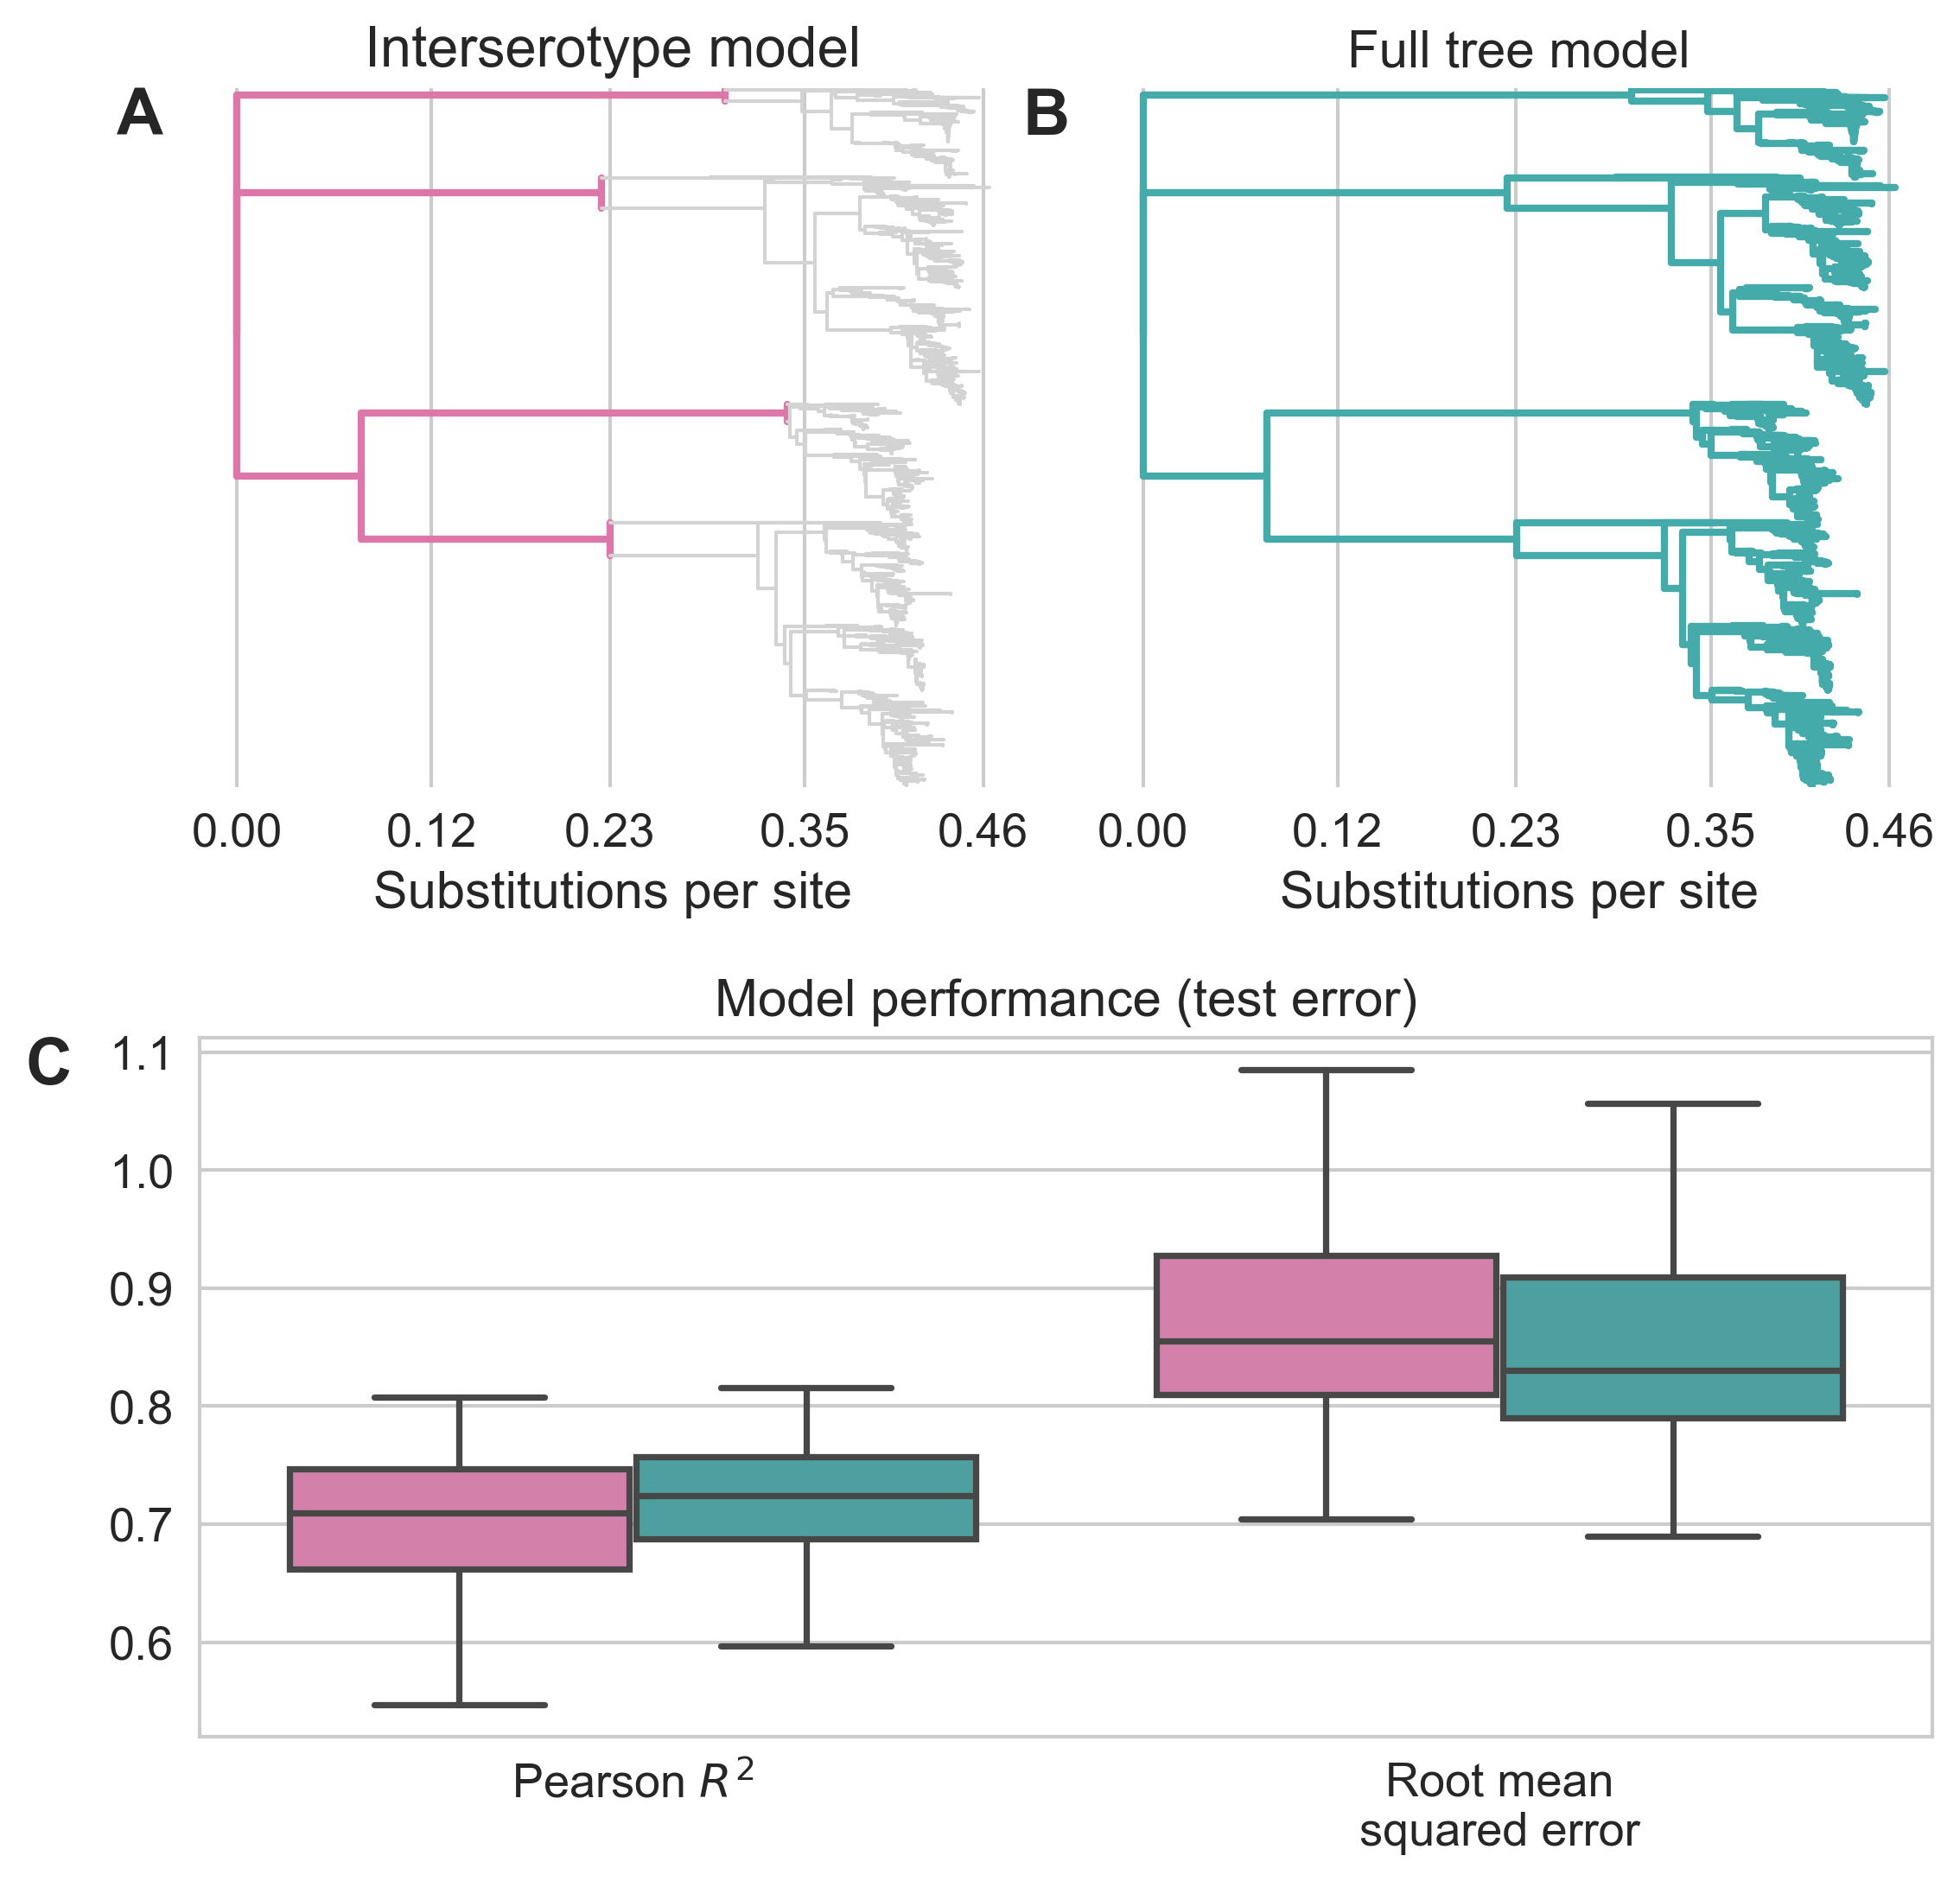
\includegraphics[width=0.75\textwidth]{../figures/png/titer_model_performance.png}
    \caption{\textbf{Titer model formulations and performance.}}
     \label{titer_model_performance}
\end{figure}


\subsection{There are at least N distinct antigenic phenotypes of dengue}
% Figure 3A: Antigenic tree


% \begin{figure}[h]
%  \centering
% \begin{subfigure}[t]{0.4\textwidth}
%     \centering
%     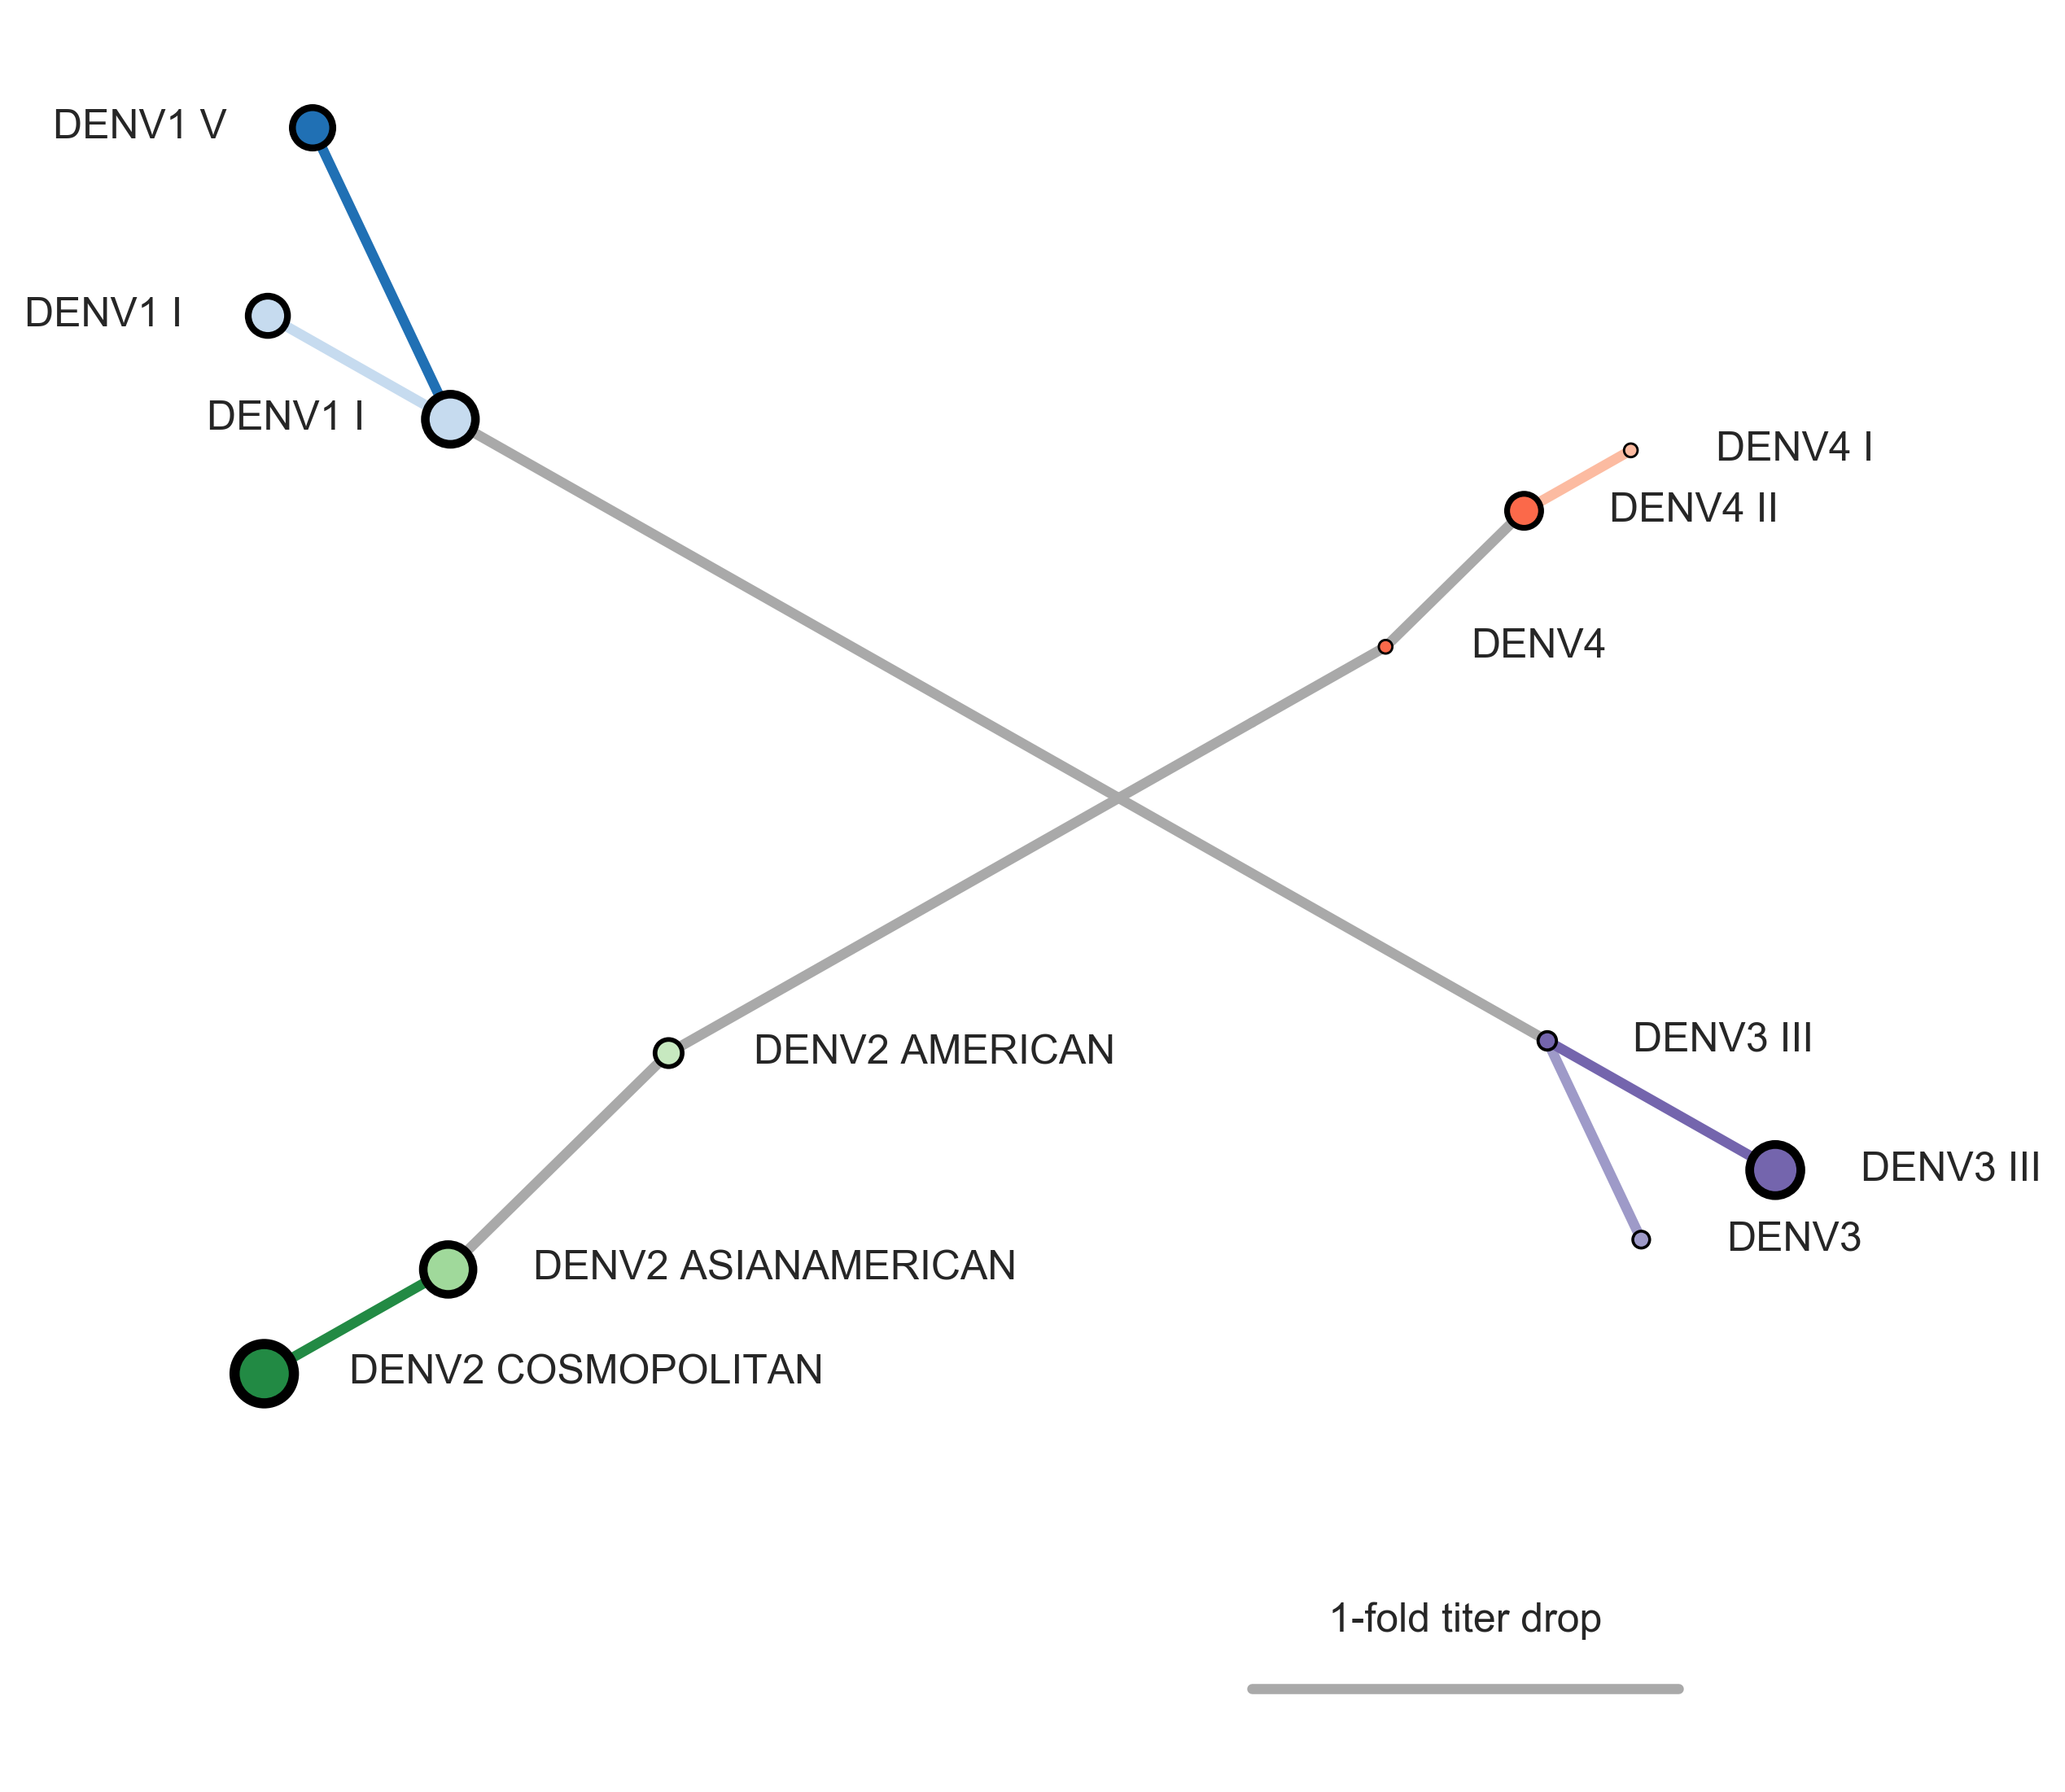
\includegraphics[width=\linewidth]{../figures/png/antigenic_tree.png}
%     \caption{\textbf{Tree of dengue antigenic phenotypes.}}
%      \label{antigenic_tree}
% \end{subfigure}
% \hfill
% \begin{subfigure}[t]{0.4\textwidth}
%     \centering
%     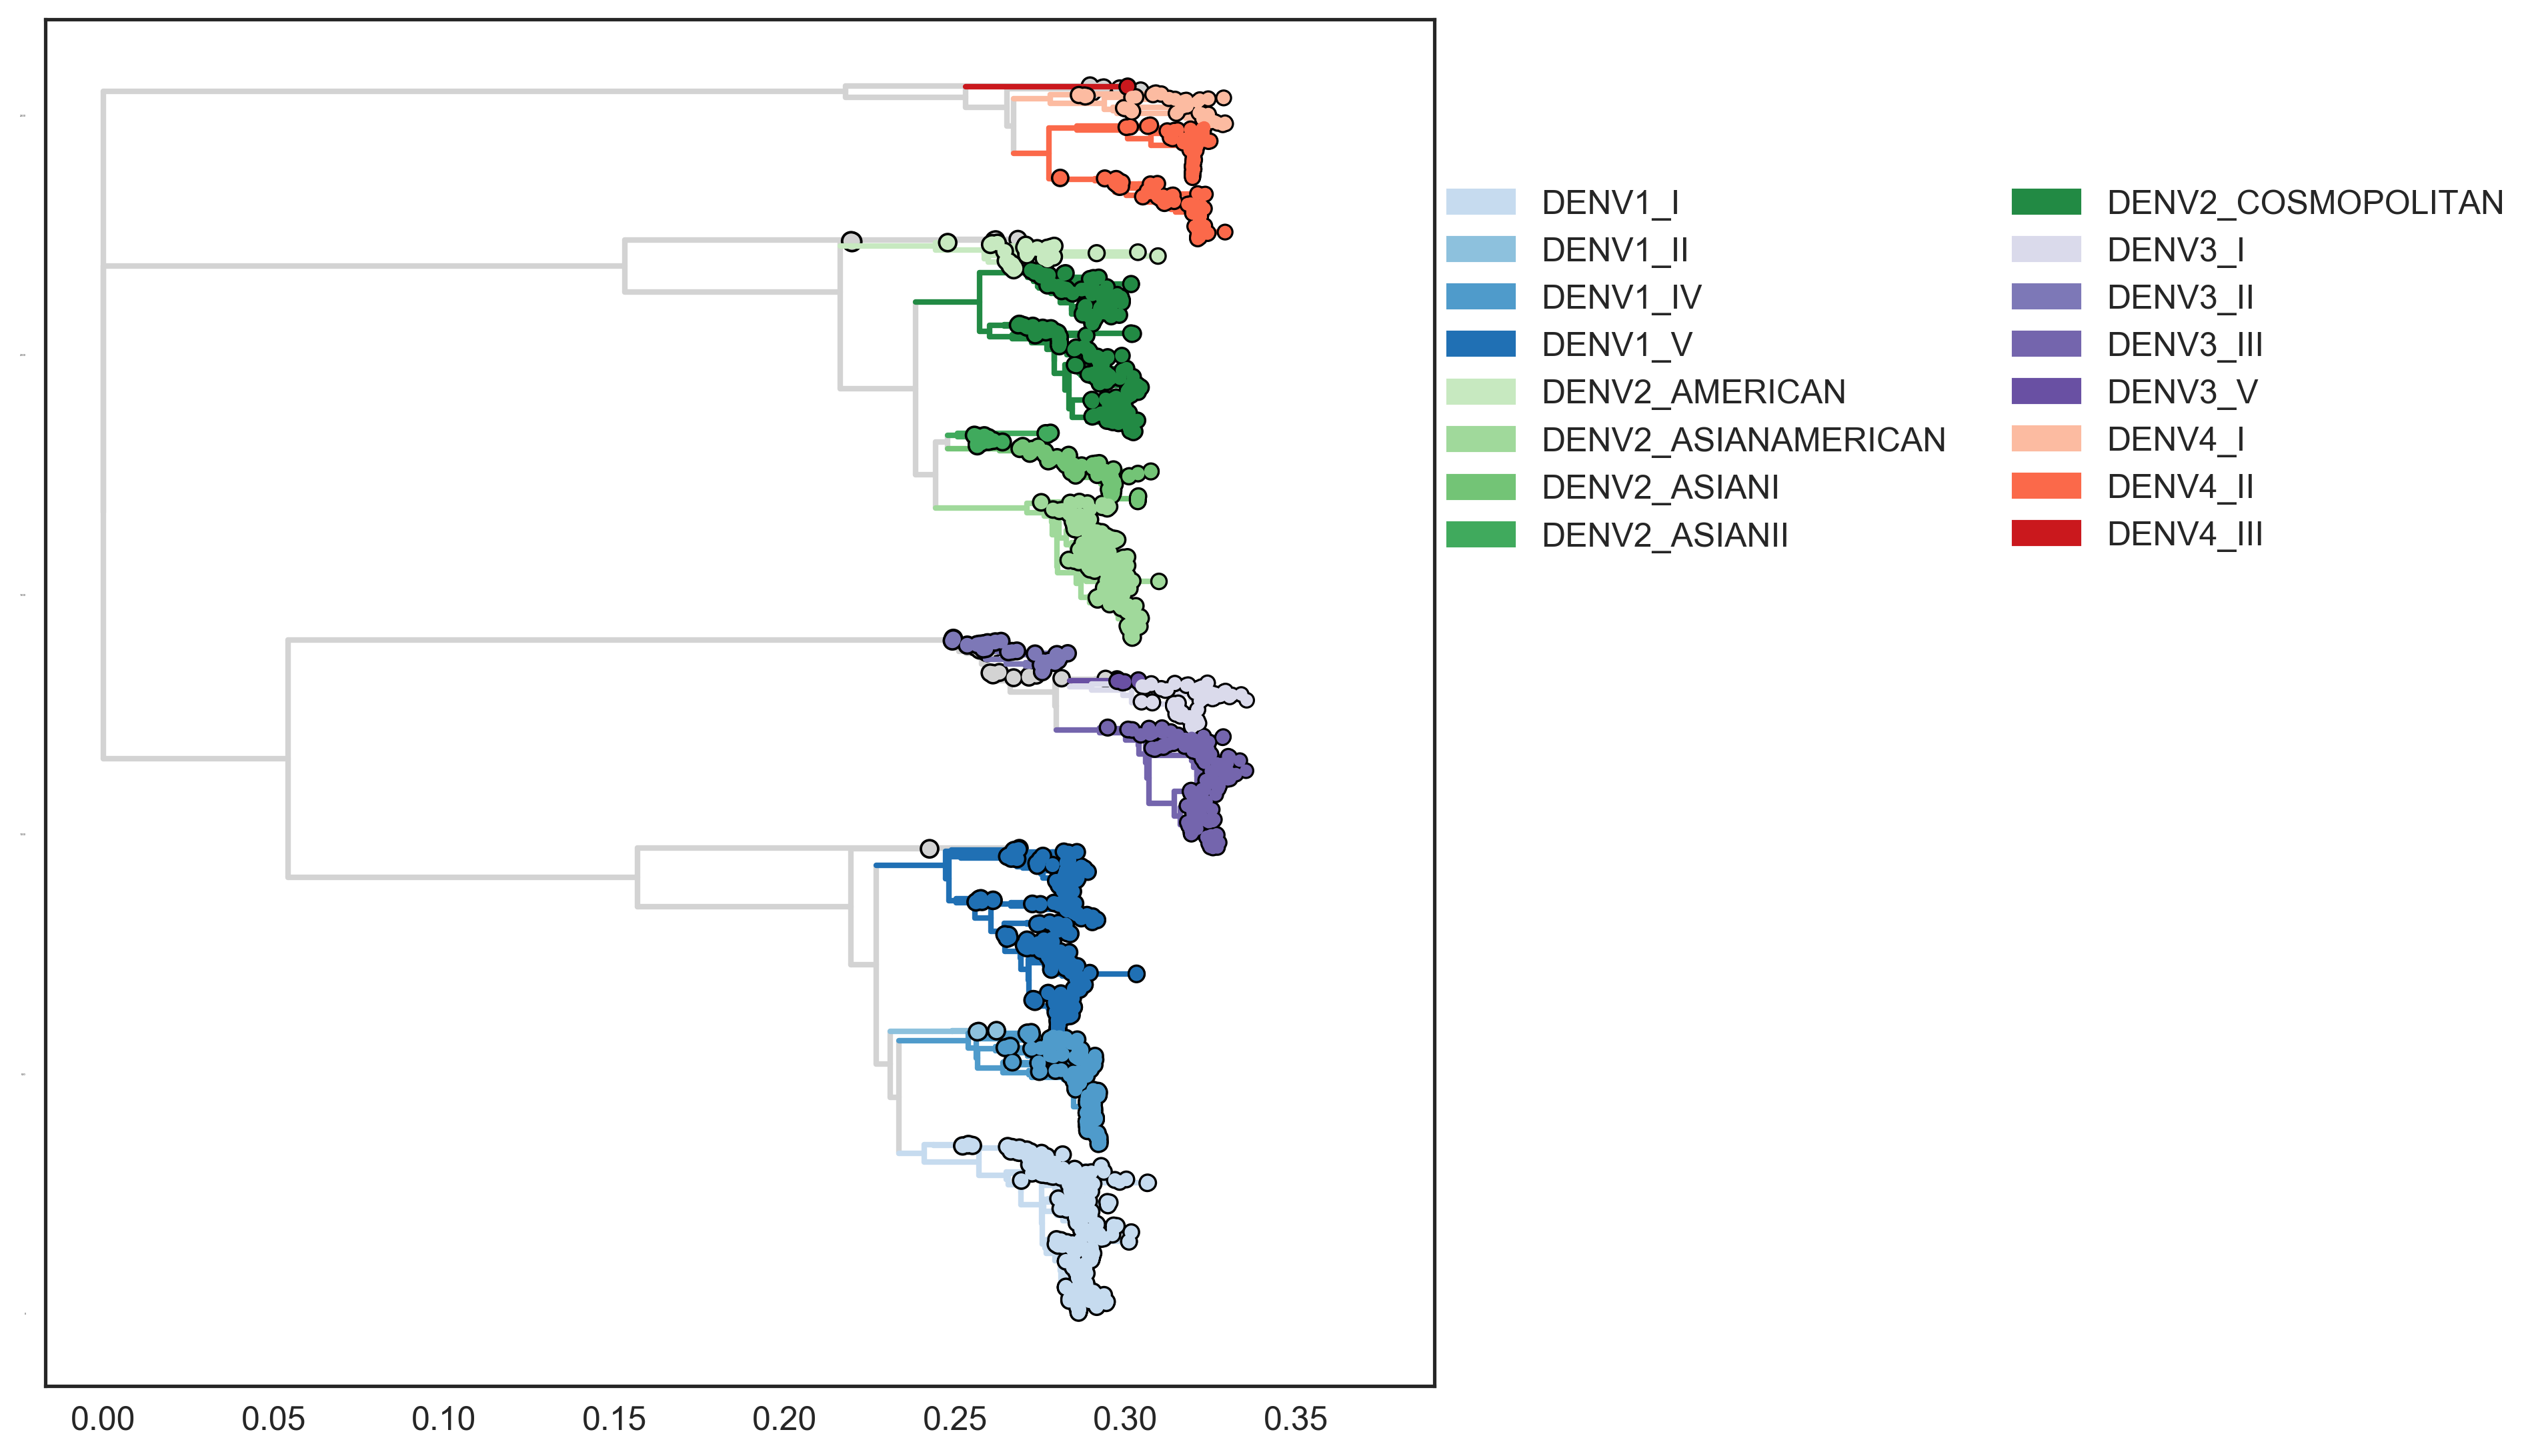
\includegraphics[width=\linewidth]{../figures/png/genotype_tree.png}
%   	\caption{\textbf{Tree of canonical dengue genotypes.}}
%   	\label{genotype_tree}
% \end{subfigure}
% \end{figure}


\subsection{Antigenic phenotypes largely correspond to canonical genotypes}
% Figure 3B: Genotype tree


\subsection{Antigenic novelty predicts serotype success}
% Figure 4: Serotype frequencies + fitness + trajectories example

\begin{figure}[h]
\centering
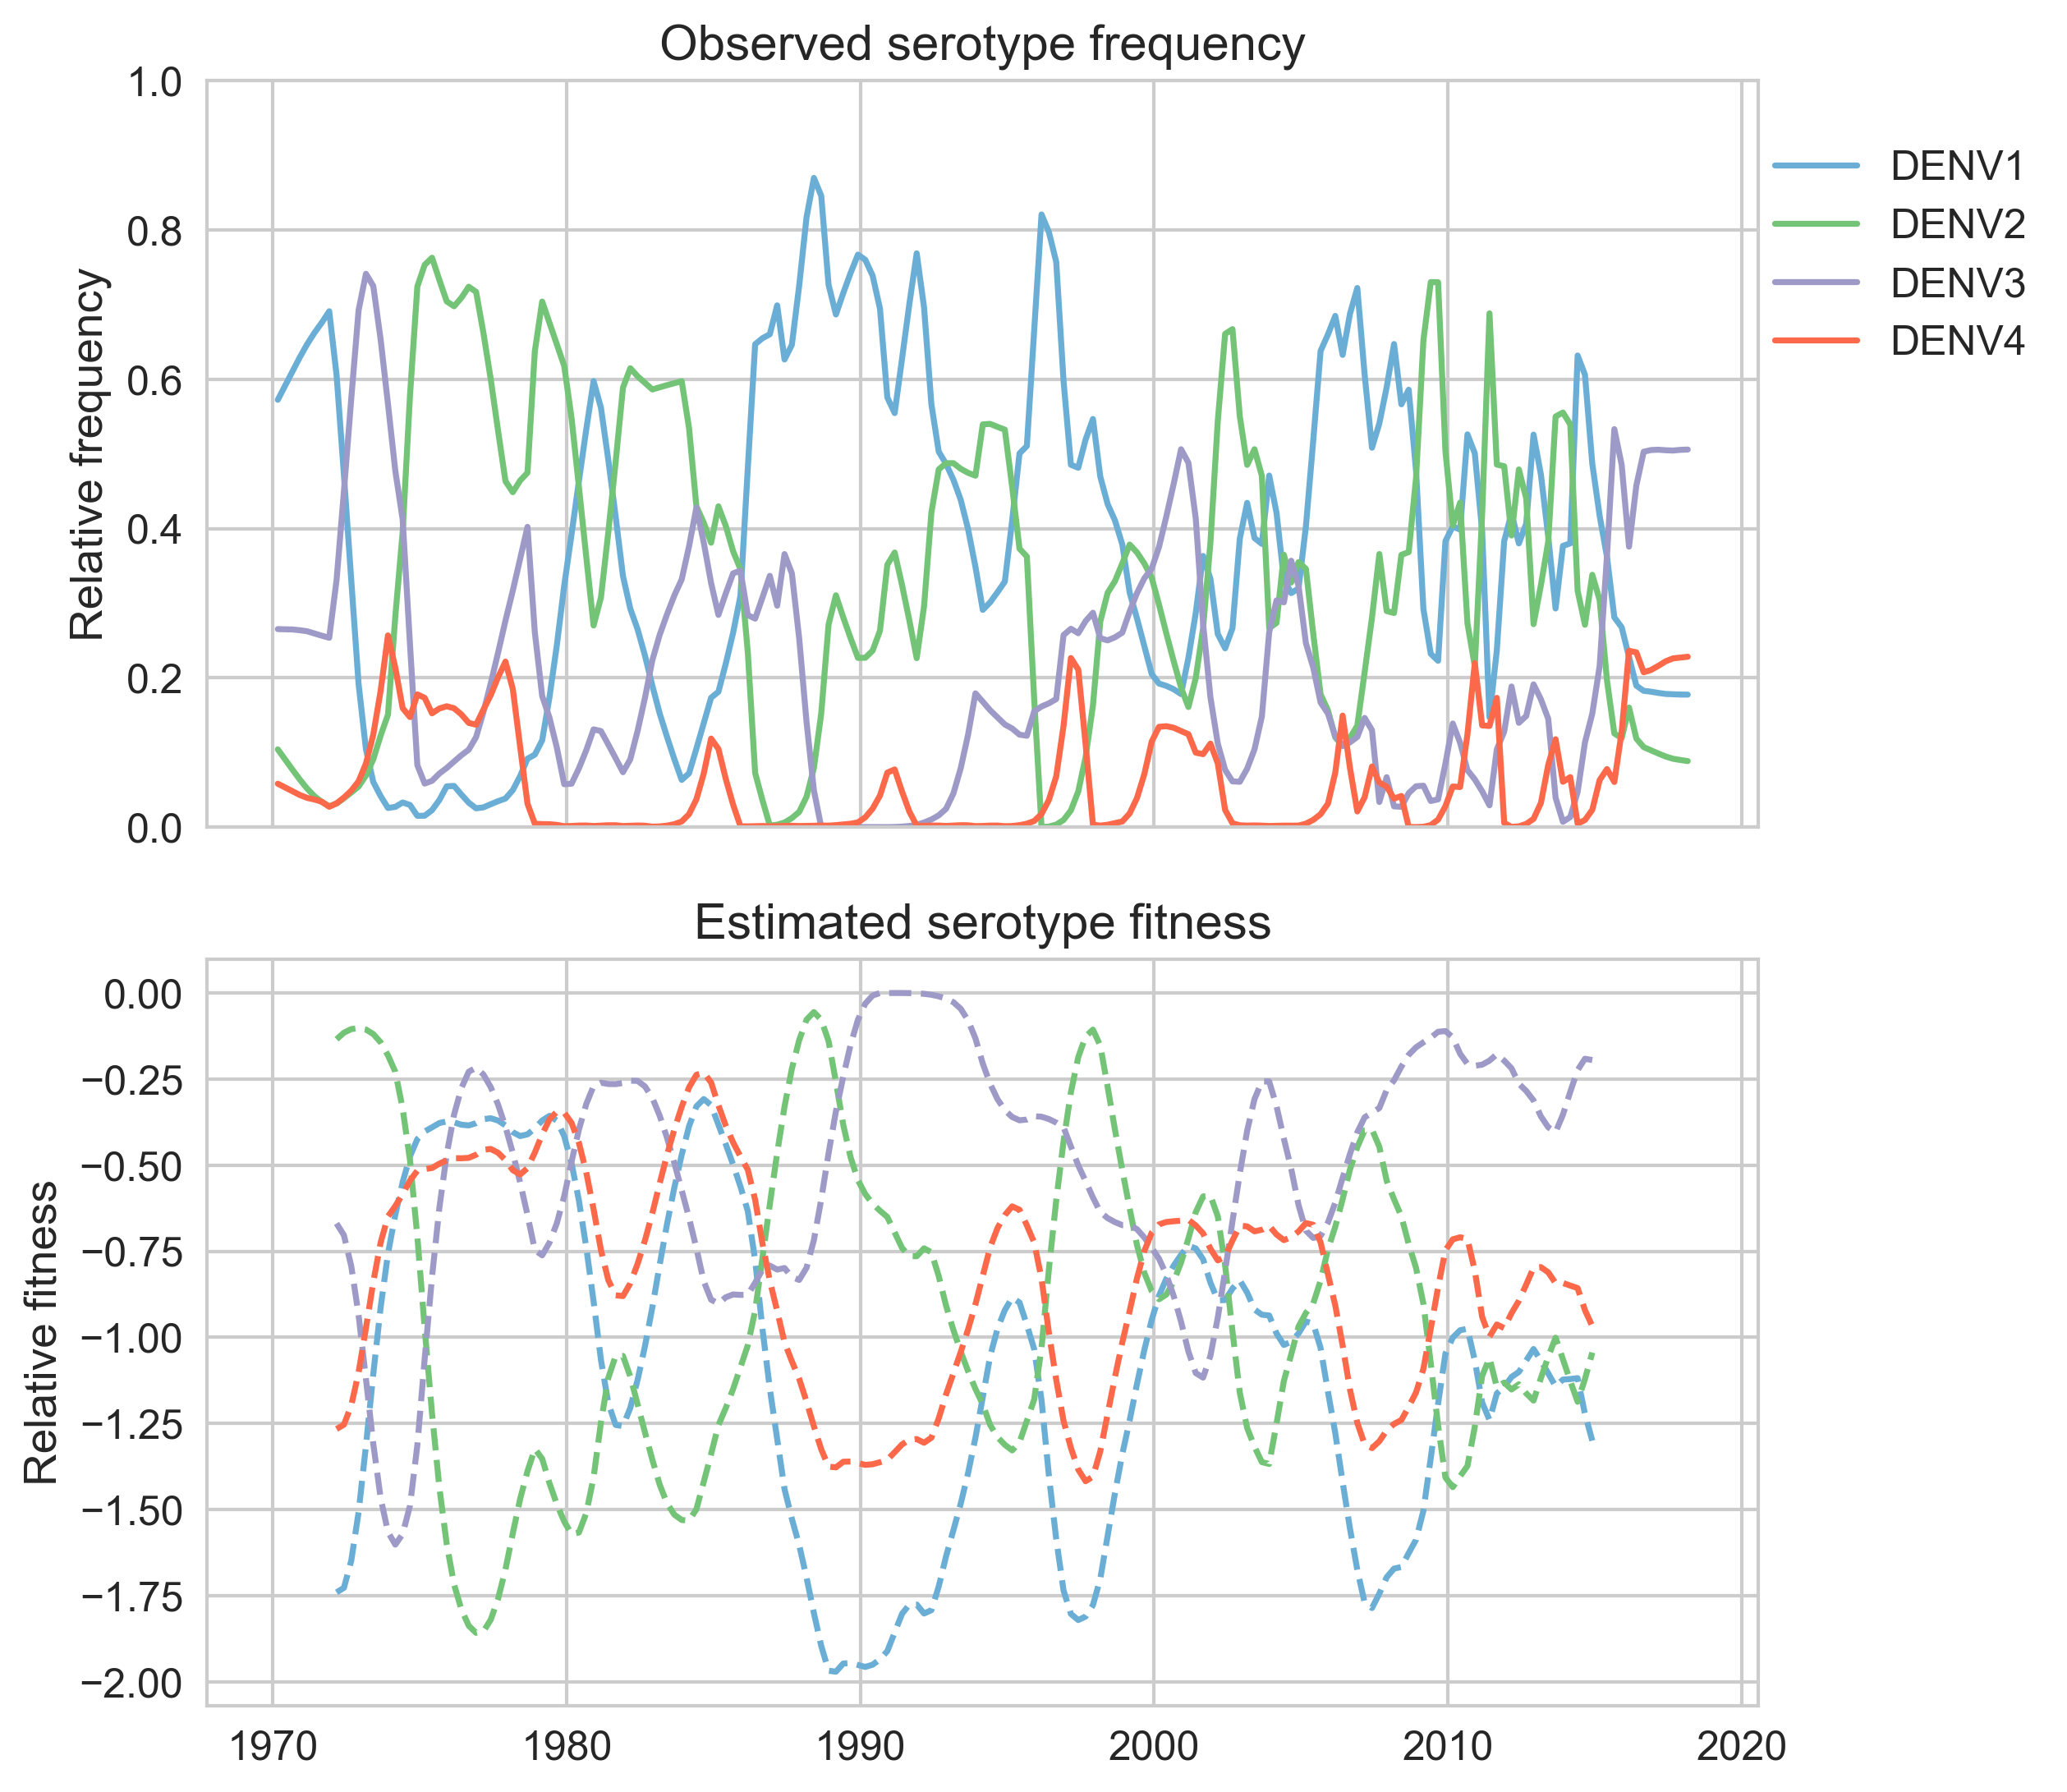
\includegraphics[width=0.75\textwidth]{../figures/png/serotype_fitness.png}
    \caption{\textbf{Relative frequencies and fitness of dengue serotypes, 1970-2015.}}
     \label{serotype_fitness}
\end{figure}


\subsection{Antigenic novelty also partially predicts genotype success}
% Figure 5: Genotype frequencies + fitness
\begin{figure}[h]
\centering
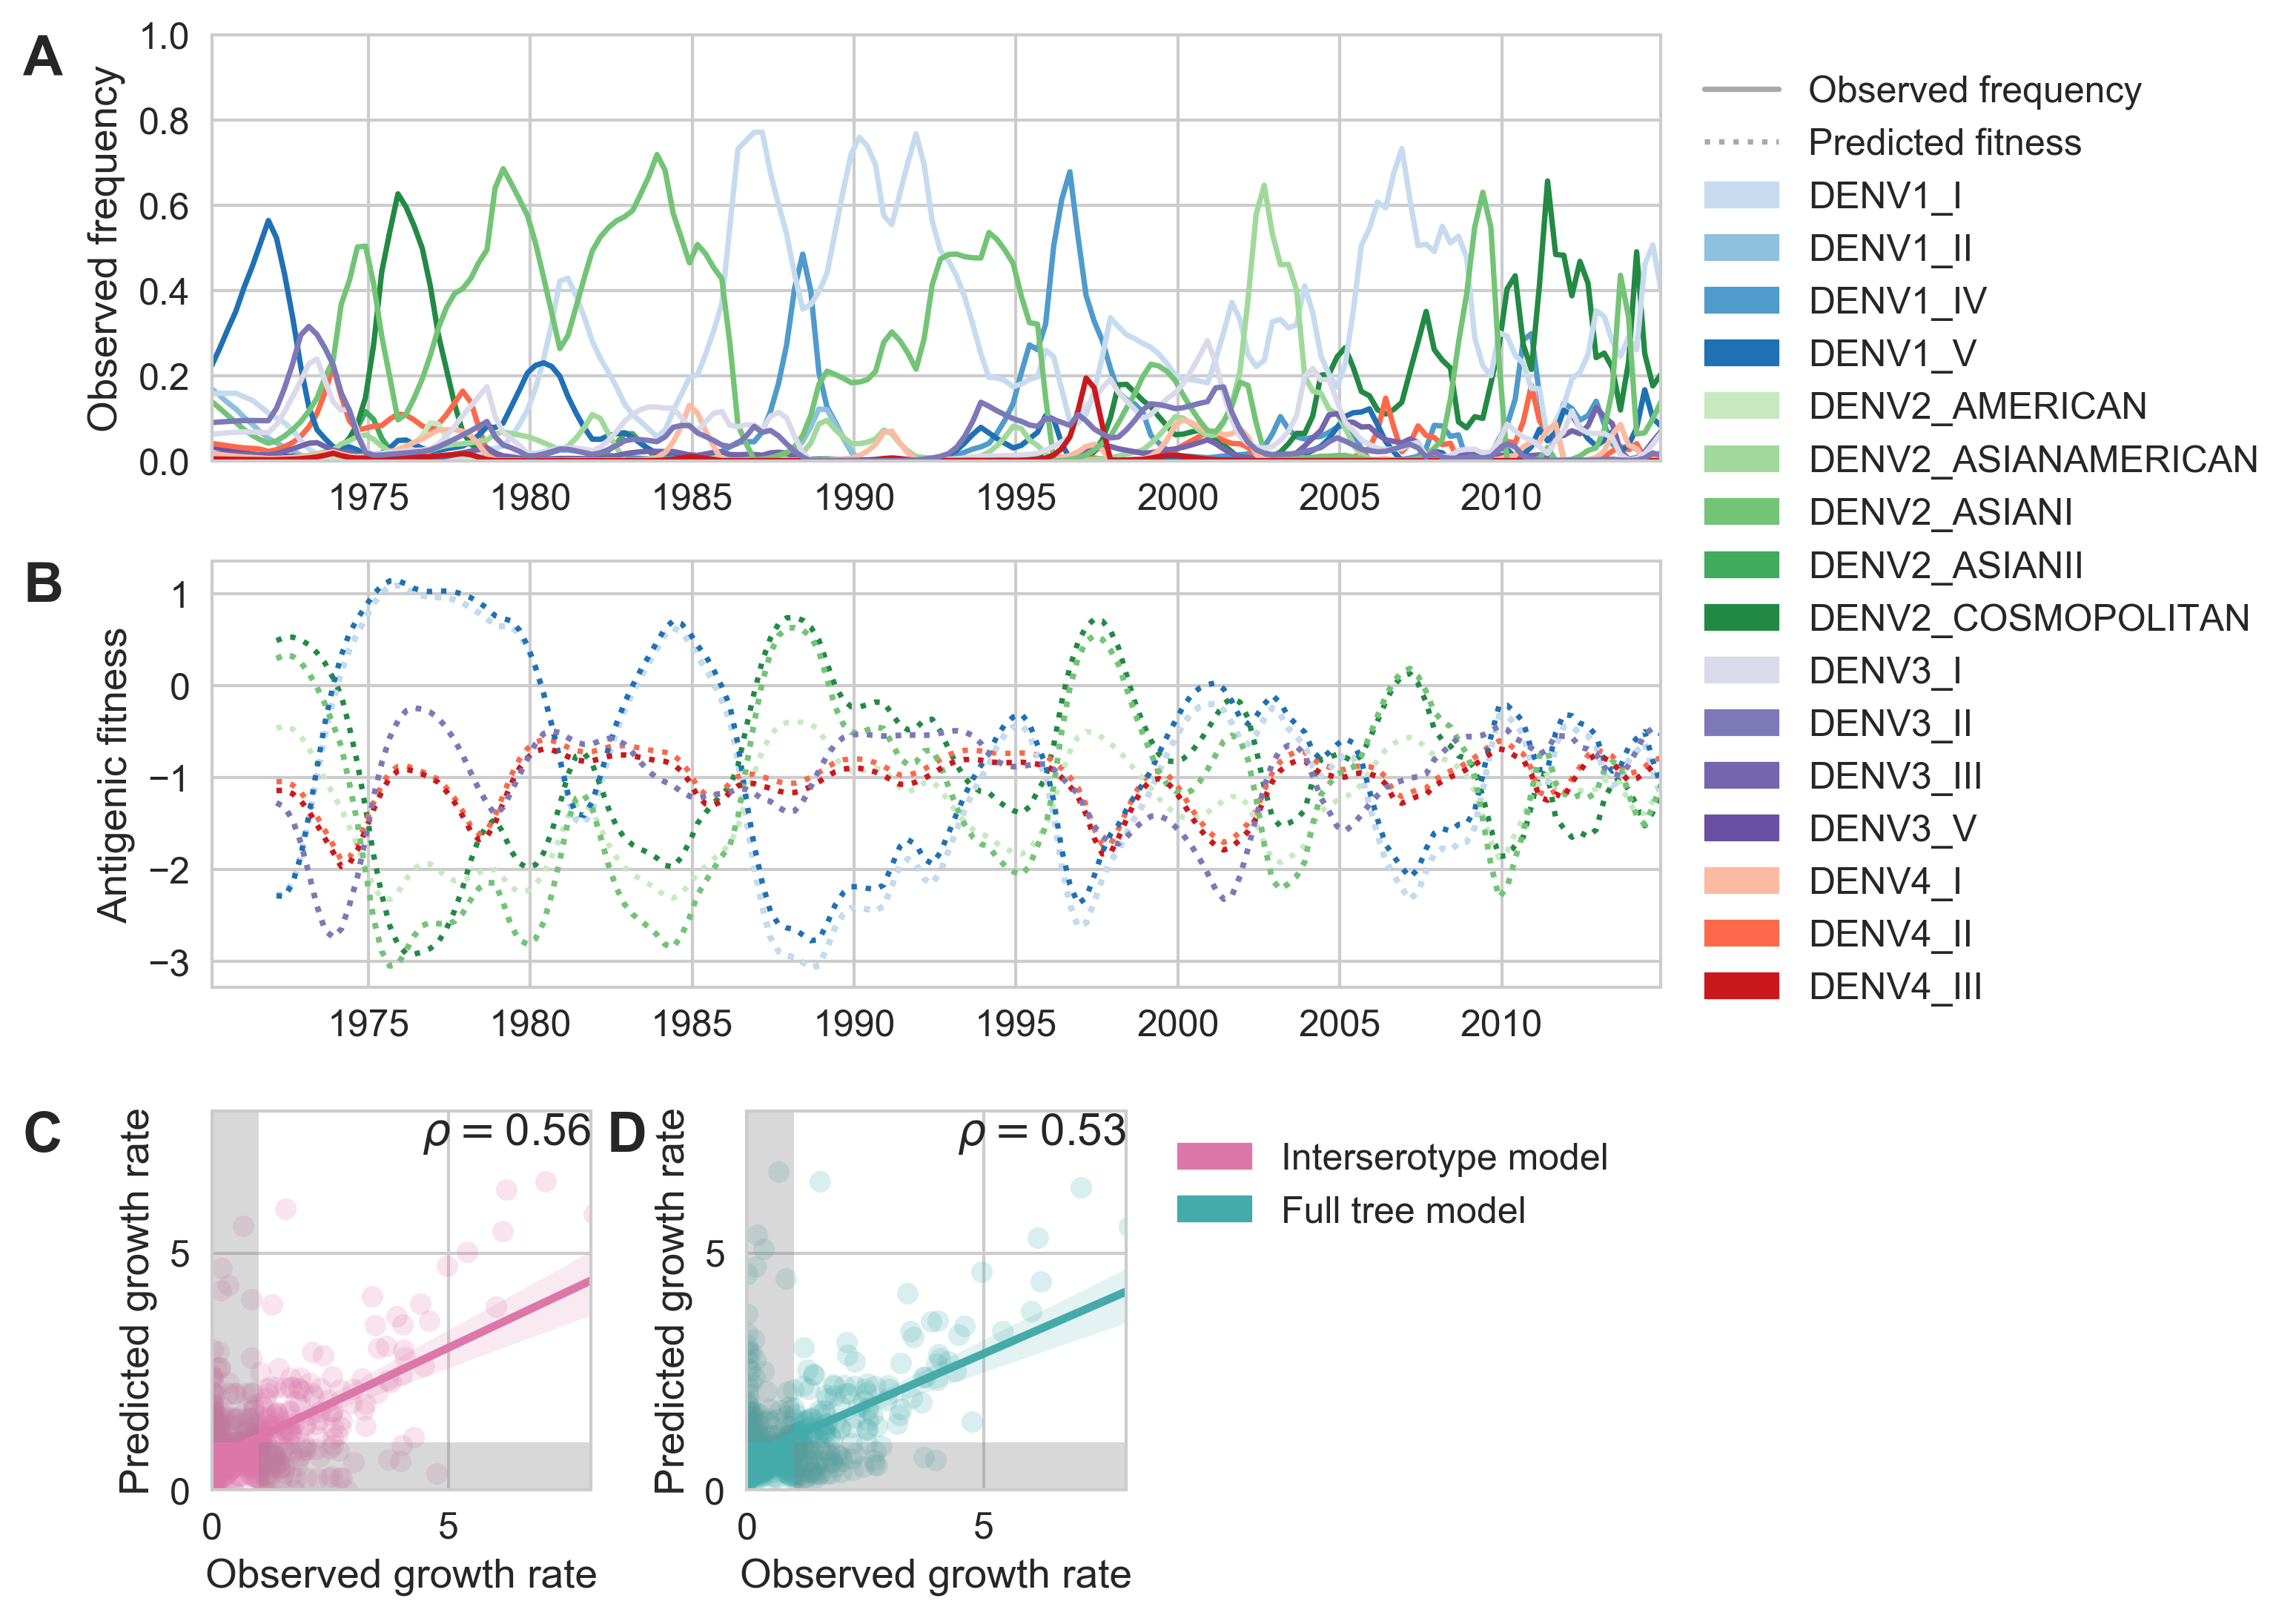
\includegraphics[width=0.75\textwidth]{../figures/png/genotype-fitness.png}
    \caption{\textbf{Relative frequencies and fitness of dengue genotypes, 1970-2015.}}
     \label{genotype_fitness}
\end{figure}


\subsection{Full-tree model does not improve predictions of genotype success}
% Figure 6: predicted vs. actual genotype growth rates (all models)
\begin{figure}[h]
\centering
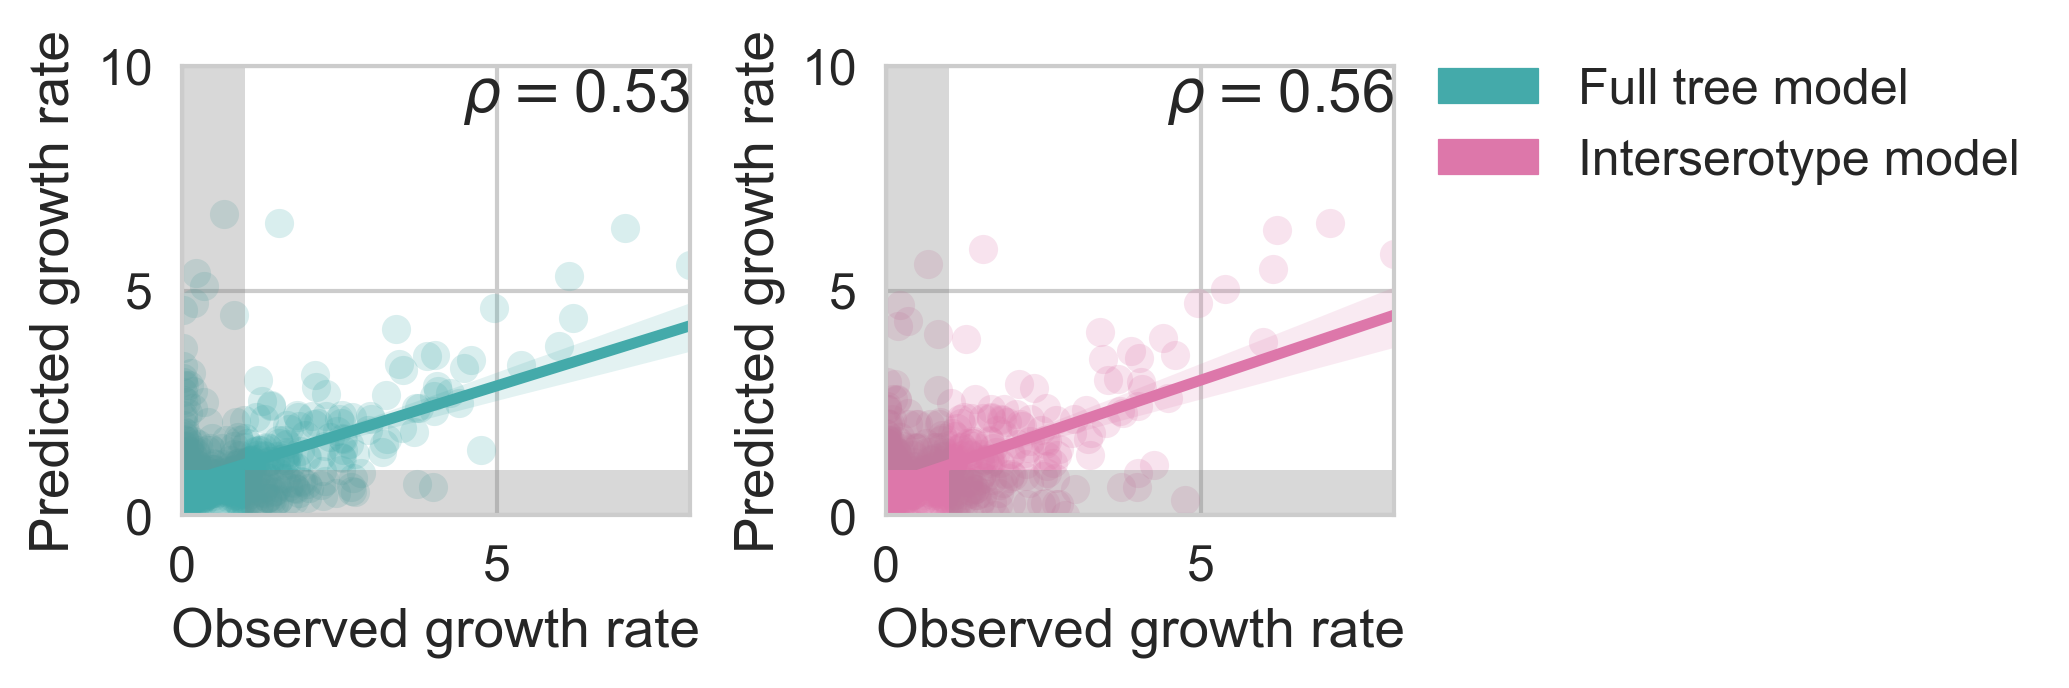
\includegraphics[width=0.75\textwidth]{../figures/png/genotype_growth_rates.png}
    \caption{\textbf{Predicted vs. actual genotype growth rates under full-tree or interserotype models of antigenic phenotype.}}
     \label{genotype_growth_rates}
\end{figure}

\begin{centering}
  \resizebox{\textwidth}{!}{
    \begin{tabular}{ l | l | l | r | r | r | r | r | r | r | r }
      \hline
      Genetic resolution & Antigenic resolution & Metric & Metric value & $\beta$ & $\gamma$ & $\sigma$ & DENV1 $f_0$ & DENV2 $f_0$ & DENV3 $f_0$ & DENV4 $f_0$ \\
      \hline
      Serotype & Interserotype & $\Delta$ SSE & 14.90 & 1.29 & 0.57 & 2.57 & 1.00 & 0.57 & 0.00 & 0.00 \\
      Serotype & Interserotype & Pearson $R^2$ & 0.62 & 1.71 & 0.57 & 2.14 & 1.00 & 0.86 & 0.00 & 0.00 \\
      \hline
      Genotype & Interserotype & $\Delta$ SSE & 14.99 & 1.71 & 0.57 & 2.57 & 1.00 & 0.57 & 0.00 & 0.00 \\
      Genotype & Interserotype & Pearson $R^2$ & 0.36 & 0.43 & 0.00 & 0.43 & 1.00 & 0.86 & 0.00 & 0.00 \\
      \hline
      Genotype & Full Tree & $\Delta$ SSE & 14.99 & 1.71 & 0.57 & 2.57 & 1.00 & 0.57 & 0.00 & 0.00 \\
      Genotype & Full tree & Pearson $R^2$ & 0.36 & 0.43 & 0.00 & 0.43 & 1.00 & 0.86 & 0.00 & 0.00 \\
      \hline
    \end{tabular}
  }
\end{centering}

\section*{Discussion}


\newpage

\section*{Methods}
\subsection*{Data}
\textbf{Sequences}\\
We downloaded all dengue virus sequences available from the Los Alamos National Lab Hemorrhagic Fever Virus Database as of March 7, 2018, that contained the full coding sequence of E (total N=12,645).
We discarded sequences which were putative recombinants, duplicates, lab strains, or which lacked an annotated sampling location and/or sampling date.
We then randomly subsampled up to 8 viruses per region, per month, preferentially including records with available titer data and longer sequences.
Our final dataset consists of 2,563 viral sequences (Supp Fig. N)

\textbf{Titers}\\
We used two publicly available plaque reduction neutralization titer (PRNT50) datasets generated by Katzelnick et al. in {[}ref{]}.
The primary dataset was generated by infecting each of N non-human primates with a unique strain of DENV.
NHP sera was drawn after 12 weeks and titered against the panel of DENV viruses.
The secondary dataset was generated by vaccinating N human trial participants with a monovalent component of the NIH DENV vaccine.
Sera was drawn after 6 weeks and titered against the same panel of DENV viruses.
As discussed in Katzelnick et al., these two datasets show similar patterns of antigenic relationships between DENV strains.
In total, our dataset includes N viruses, N sera, and N measurements.

\subsection*{Titer Model}
We normalize measured titers between virus i and serum j, $T_{ij}$, relative to autologous titers: $$T_{ij} = log_2(T_{ii}) - log_2(T_{ij})$$
To predict unmeasured titers, we employ the 'tree model' from Neher et al. and implemented in Nextstrain, which assumes that antigenic evolution is driven by underlying genetic evolution.
Observed titer drops are mapped to branches in the viral phylogeny after correcting for overall virus avidity, $v_i$, and serum potency, $p_j$ (row and column effects, respectively):
$$\hat{T}_{ij} \approx T_{ij} = \sum_{b \in path(i,j)} d_b + v_i + p_j$$
where $d_b$ is the titer drop assigned to each branch, $b$, in the phylogeny.
We randomly withhold 10\% of titer measurements as a test set.
We use the remaining 90\% of titer measurements as a training set to learn values for virus avidity, serum potency, and branch effects.
As in Neher et al., we formulate this as a convex optimization problem and solve for these parameter values to minimize the cost function:
$$C = \sum_{i,j} (\hat{T}_{ij} - T_{ij})^2 + \lambda \sum_{b} d_b + \gamma \sum_{i} v_i^2 + \delta \sum_{i} p_i^2$$
Respectively, these terms represent the squared training error; an L1 regularization term on branch effects, such that most values of $d_b = 0$; and L2 regularization terms on virus avidities and serum potencies, such that they are normally distributed.
These parameter values are then used to predict the titer distance between all pairs of viruses, $i$ and $j$, in the phylogeny.
We assess performance by comparing predicted to known titer values in our test data set, and present test error (aggregated from 10-fold cross-validation) throughout the manuscript.

\subsection*{Viral Clade Dynamics}

\textbf{Empirical Clade Frequencies}\\
As discussed in Neher et al and Lee et al, we estimate empirical clade frequencies from 1970 to present based on observed relative abundance of each clade in the "slice" of the phylogeny corresponding to each quarterly timepoint.

Briefly, the frequency trajectory of each clade in the phylogeny is modeled according to a Brownian motion diffusion process discretized to three-month intervals.
Relative to a simple Brownian motion, the expectation includes an "inertia" term that adds velocity to the diffusion and the variance includes a term $x(1-x)$ to scale variance according to frequency following a Wright-Fisher population genetic process.
This results in the following diffusion process:
$$x(t+dt) = \mathcal{N}(x(t) + \epsilon dx, dt \sigma^2 x(t) (1-x(t)))$$

with `volatility' parameter $\sigma^2$.
The term $dx$ is the increment in the previous timestep, so that $dx = x(t) - x(t-dt)$.
We used $\epsilon = 0.7$ and $\sigma = 2.0$ to maximize fit to empirical trajectory behavior.

We also include an Bernoulli observation model for clade presence / absence among sampled viruses at timestep $t$.
This observation model follows
$$f(x,t) = \Pi_{v \in V} x(t) \Pi_{v \notin V} (1-x(t))$$
where $v \in V$ represents the set of viruses that belong to the clade and $v \notin V$ represents the set of viruses that do not belong to the clade.
Each frequency trajectory is estimated by simultaneously
maximizing the likelihood of the process model and the likelihood
of the observation model via adjusting frequency trajectory $\vec{x} = (x_1, ... x_n)$.

\textbf{Population Immunity}\\
For antigenically diverse pathogens, antigenic novelty represents a fitness advantage.
This means that strains that are antigenically distinct from previously-circulating strains are able to access more susceptible hosts, allowing the antigenically novel lineage to expand.
We adapt a simple deterministic model from Luksza and Lassig to directly quantify dengue antigenic novelty and its impact on viral fitness.
We quantify population immunity to virus $i$ at time $t$, $P_i(t)$, as a function of which clades have recently circulated in the past $N$ years, and how antigenically similar each of these clades is to virus $i$:
$$P_i(t) = \sum_{n=1}^{n=N} (w(n)  \sum_{j} x_j(t-n) * C( D_{ij}))$$
Where $D_{ij}$ is the antigenic distance between $i$ and each non-overlapping clade $j$, $n$ is the number of years since exposure, and $x_j(t-n)$ is the relative frequency of $j$.
Waning immunity is modeled as a non-negative linear function of time:
$$w(n) = max(-\gamma n + 1, 0)$$
The relationship between titers and the probability of protection, $C$, is also assumed to be linear and non-negative, such that:
$$C(D_{ij}) = max(-\sigma D_{ij} + 1, 0)$$

We model the effects of population immunity, $P_i(t)$, on viral antigenic fitness, $f_i(t)$, as:
$$f_i(t) = f_0-\beta P_i(t)$$
where $\beta$ and $f_0$ are fit parameters representing the slope of the linear relationship between immunity and fitness, and the intrinsic relative fitness of each serotype, respectively.

\textbf{Frequency Predictions}\\
Similar to the model implemented in Luckzsa and Lassig, we estimate predicted clade frequencies at time $t + dt$ as
$$\hat{x_i}(t+dt) = \frac{x_i(t) e^{f_i(t) dt}}{\sum_{i}x_i(t)}$$
for short-term predictions (where $dt < 1$).

For long-term predictions, we must account for immunity accrued at each intermediate timepoint between $t$ and $dt$.
We divide the interval between $t$ and $dt$ into a total of $U$ 3 month timepoints, $[t+u, t+2u, ... t+U]$, where $t+U=dt$.
We then compound immunity based on predicted clade frequencies at each intermediate timepoint:
$$\hat{x_i}(t+u) = x_i(t)e^{f_i(t) u}$$
$$\hat{x_i}(t+2u) = \hat{x_i}(t+u) e^{f_i(t+u)u}$$
$$...$$
$$\hat{x_i}(t+U) = x_i(t) e^{f_i(t)u} e^{f_i(t+u)u} e^{f_i(t+2u)u} ... e^{f_i(t+U)u}$$
$$\hat{x_i}(t+dt) = \hat{x_i}(t+U) = x_i(t) e^{\sum_{u}f_i(t+u)u}$$

We can then calculate clade growth rates, defined as the fold-change in relative clade frequency between time $t$ and time $t+dt$:
$$\frac{\hat{x_i}(t+dt)}{x_i(t)}$$

\textbf{Null model and model performance}\\
To quantify the impact of antigenic fitness on DENV clade success, we compare our antigenically-informed model to a null model wherein all strains have equal antigenic fitness at all timepoints:
$$f_i^{null}(t) = 0$$
$$\hat{x_i}^{null}(t+dt) = x_i(t) e^0 = x_i(t)$$

For both the null model and the antigenically-informed model, we can assess predictive power as the sum of squared error between predicted and empirical clade growth rates:
$$SSE = \sum_{i,t} (\frac{\hat{x_i}(t+dt)}{x_i(t)} - \frac{\hat{x_i}^{null}(t+dt)}{x_i(t)})^2$$

We can then estimate how much more error is present in the null model than the antigenically-informed model:
$$\Delta SSE = SSE^{null} - SSE^{model}$$

Our frequency prediction model has a total of 8 free parameters:
\begin{table}[h!]
  \begin{center}
    \label{tab:table1}
    \begin{tabular}{c|l}
      $\beta$ & Slope of linear relationship between population immunity and viral fitness\\
      $\gamma$ & Slope of linear relationship between titers and probability of protection\\
      $\sigma$ & Proportion of titers waning each year since primary infection\\
      $f_{s0}$ & Relative intrinsic fitness of each serotype ($f_0 = 1$ for DENV1)\\
      $N$ & Number of years of previous immunity that contribute to antigenic fitness\\
      $dt$ & Number of years in the future to predict clade frequencies\\
    \end{tabular}
  \end{center}
\end{table}

For each dataset, we jointly fit these parameters to maximize $\Delta SSE$.

\subsection*{Data availability}
Sequence and titer data, as well as all code used for analyses and figure generation, is publicly available at \href{https://github.com/blab/dengue}{github.com/blab/dengue}.

\section*{Acknowledgements}
We would like to thank \_ for useful discussion and advice.
SB is supported by \_.
TB is a Pew Biomedical Scholar and is supported by NIH R35 GM119774-01 and \_.

% \bibliographystyle{mbe}
% \bibliography{mers-structure}

\newpage

% SUPPLEMENT STARTS HERE

% \setcounter{figure}{0}
% \setcounter{table}{0}
% \renewcommand{\thefigure}{S\arabic{figure}}
% \renewcommand{\thetable}{S\arabic{table}}
%
% \begin{longtable}{ | r | l | p{2cm} | l | l | } % COLUMN FORMATS
%
%   \caption{TABLE CAPTION HERE} \label{TABLE LABEL HERE} \\
%   \endfirsthead
%
%   1 & KSA-378 & KJ713296 & camel & 2013-11 \\
%   2 & KSA-363 & KJ713298 & camel & 2013-11 \\
%   3 & KSA-503 & KJ713297 & camel & 2013-11 \\
%
% \end{longtable}

% \begin{figure}[h]
% \centering
% 	% \includegraphics[width=0.65\textwidth]{figures/mers_exploded.png}
% 	\caption{\textbf{SUP FIGURE 1 TITLE }
% SUPP FIGURE 1 CAPTION
% 	}
% 	\label{SUP_FIGURE_1_LABEL}
% \end{figure}


\end{document}
